\documentclass{ximera}

\newcommand{\RR}{\mathbb R}
\renewcommand{\d}{\,d}
\newcommand{\dd}[2][]{\frac{d #1}{d #2}}
\renewcommand{\l}{\ell}
\newcommand{\ddx}{\frac{d}{dx}}
\newcommand{\dfn}{\textbf}
\newcommand{\eval}[1]{\bigg[ #1 \bigg]}


\outcome{Use the ratio test to determine if a series diverges or converges.}

\title[Dig-In:]{The ratio test}

\begin{document}
\begin{abstract}
Some infinite series can be compared to geometric series.
\end{abstract}
\maketitle

As mathematicians, we are explorers. We explore the implications of
seemingly simple quantitative facts. 

\begin{exploration}
Consider the infinite series $\sum_{k=0}^\infty \frac{k}{2^k}$. 

Let $a_k = \answer[given]{\frac{k}{2^k}}$ be the formula for the terms in sequence whose sum we are trying to find.  We can observe something interesting when $k$ is large by looking at the ratio $\left|\frac{a_{n+1}}{a_n}\right|$.

Notice that by treating the division by $a_k$ as multiplication by its reciprocal, 

\[
\lim_{k \to \infty} \left|\frac{a_{n+1}}{a_n}\right| = \lim_{k \to \infty} \frac{k+1}{2^{k+1}} \cdot \frac{2^k}{k}.
\]

After rearranging a little, we have

\[
\lim_{k \to \infty} \left|\frac{a_{n+1}}{a_n}\right| = \lim_{k \to \infty} \frac{k+1}{k} \cdot \frac{2^k}{2^{k+1}},
\]

and we can now finish computing the limit.

\[
\lim_{k \to \infty} \left|\frac{a_{n+1}}{a_n}\right| = \lim_{k \to \infty} \frac{k+1}{k} \cdot \frac{\cancel{2^k}}{\cancel{2^k} \cdot 2^1} = \answer[given]{\frac{1}{2}}.
\]

Thus, when $k$ is large, $a_{k+1}$ is pretty close to
\wordChoice{\choice[correct]{half}\choice{double}} of $a_{k}$.  
So, when we choose a very large whole number $N$, $a_{N+1}$ should be approximately $\frac{1}{2} a_N$, and this should occur for \emph{all} successive terms in the sequence $\{a_k\}$.  That is, 

\[
a_{k+1} \approx  \frac{1}{2} \cdot a_k
\]
for all $k>N$.

We can then observe the following.
\begin{align*}
  a_{N+1} &\approx  \frac{1}{2} \cdot a_N \\
  a_{N+2} &\approx  \frac{1}{2} \cdot a_{N+1}  \approx \frac{1}{2} \cdot \left(\frac{1}{2} \cdot a_N\right) = \answer[given]{\left(\frac{1}{2}\right)^2} \cdot a_N \\
  a_{N+3} &\approx  \frac{1}{2} \cdot a_{N+2}  \approx \frac{1}{2} \cdot \left( \left(\frac{1}{2}\right)^2 \cdot a_N\right) = \answer[given]{\left(\frac{1}{2}\right)^3} \cdot a_N \\
\vdots
\end{align*}

We thus have that 

\[
\sum_{k=N}^{\infty}  \frac{k}{2^k} \approx \sum_{k=N}^{\infty} \left(\frac{1}{2}\right)^k \cdot a_N.
\]
In words, the tail of the sequence $\{a_k\}_{k=N}$ is ``approximately'' a geometric series with ratio $\frac{1}{2}$.

\begin{question}
Does a geometric series with ratio $\frac{1}{2}$ converge or diverge?
\begin{prompt}
  \begin{multipleChoice}
    \choice[correct]{converge}
    \choice{diverge}
  \end{multipleChoice}
\end{prompt}
\begin{question}
  Given your answer above, do you suspect that the original sum
  $\sum_{k=0}^\infty \frac{k}{2^k}$ converges or diverges?
  \begin{prompt}
    \begin{multipleChoice}
      \choice[correct]{converge}
      \choice{diverge}
    \end{multipleChoice}
  \end{prompt}
\end{question}
\end{question}
\end{exploration}

As it turns out, the above ideas can be formalized and written as a theorem.  The proof of
this theorem is slightly beyond the scope of the course, but really only involves introducing formal mathematical language to make the above observations precise.

\begin{theorem}[The Ratio Test]\index{ratio test}
Consider $\sum_{k=k_0}^\infty a_k$ and set 

\[
L = \lim_{n \to \infty} \left| \frac{a_{n+1}}{a_n} \right|. 
\]

\begin{itemize}
  \item If $0 \leq L < 1$, then the series converges.
  \item If $L>1$ or $r$ is infinite, then the series diverges.
  \item If $L = 1$, the test is inconclusive; the series could diverge or converge.
  \end{itemize}
\end{theorem}

Note that this is easy to remember if you just use the following heuristic.
\begin{quote}
  If the ratio test gives a limit of $r \neq 1 $, then the series is like a
  geometric series of ratio $r$.
\end{quote}
The case of $r=1$ is an ``edge'' case, and can go either way, which we will demonstrate with specific examples in a bit.

Now that you have the basic idea, we give examples showing the following.
\begin{itemize}
\item Convergence by the ratio test.
\item Divergence by the ratio test.
\item A divergent series for which the ratio test is inconclusive.
\item A convergent series for which the ratio test is inconclusive.
\end{itemize}
In these examples, pay attention to how the ratio of different types of terms behave and simplify.



\begin{example}
  Consider $  \sum_{k=4}^\infty \frac{2^k}{k!}$.  Discuss the convergence of this series.
  \begin{explanation}
    We will attempt to use the ratio test. Setting $a_n = \frac{2^n}{n!}$, we compute
\begin{align*}
    \lim_{n \to \infty} \frac{a_{n+1}}{a_n} &=  \lim_{n \to \infty} \frac{2^{n+1}}{(n+1)!} \cdot \frac{n!}{2^n} \\
    &=  \lim_{n \to \infty} \frac{2^{n+1}}{2^n}  \cdot \frac{n!}{(n+1)!} \\
    &=  \lim_{n \to \infty} \frac{\cancel{2^n}\cdot 2^1}{\cancel{2^n}}  \cdot \frac{\cancel{n!}}{(n+1) \cdot \cancel{n!} } \\
    &= \answer[given]{0}
\end{align*}

    So, the ratio test
	 \wordChoice{
	   \choice[correct]{ guarantees that $  \sum_{k=4}^\infty \frac{2^k}{k!}$ is convergent}
	   \choice{ guarantees that $\sum_{k=4}^\infty \frac{2^k}{k!}$ is divergent}
	   \choice{gives no information in this case, but we know the series is convergent through some other method}
	   \choice{gives no information in this case, but we know the series is divergent through some other method}}.	
	 \begin{hint}
	 
	   So the series is convergent by the ratio test.  Note that
           this shows that $k!$ grows \textbf{much faster} than the
           exponential function $2^k$.
	 \end{hint}
  \end{explanation}
\end{example}

\begin{example}
  Consider $  \sum_{k=1}^\infty \frac{5^{1+k}}{k \cdot 2^{2k+1}}$.  Discuss the convergence of this series.
  \begin{explanation}
    We will attempt to use the ratio test. Setting $a_n =
    \frac{5^{1+n}}{n \cdot  2^{2n+1}}$, we compute  
\begin{align*}
    \lim_{n \to \infty} \left|\frac{a_{n+1}}{a_n}\right| &= \lim_{n \to \infty} \frac{5^{n+2}}{(n+1)2^{2(n+1)+1}} \cdot  \frac{n 2^{2n+1}}{5^{n+1}}\\
	&=\lim_{n \to \infty} \frac{5^{n+2}}{5^{n+1}} \cdot  \frac{2^{2n+1}}{2^{2n+3}} \cdot \frac{n}{n+1}\\
	&=\lim_{n \to \infty} \frac{\cancel{5^{n+1}}\cdot 5^1}{\cancel{5^{n+1}}} \cdot  \frac{\cancel{2^{2n+1}}}{\cancel{2^{2n+1}}\cdot 2^2} \cdot \frac{n}{n+1}\\
	&=\lim_{n \to \infty} \frac{5}{4} \cdot \frac{n}{n+1}\\
	&=\frac{5}{4}
      \end{align*}	
      
    So, the ratio test
    \wordChoice{
      \choice{ guarantees that $  \sum_{k=1}^\infty \frac{5^{1+k}}{k \cdot 2^{2k+1}}$ is convergent}
      \choice[correct]{ guarantees that $  \sum_{k=1}^\infty \frac{5^{1+k}}{k \cdot 2^{2k+1}}$ is divergent}
      \choice{gives no information in this case, but we know the series is convergent through some other method}
      \choice{gives no information in this case, but we know the series is divergent through some other method}}. 
  \end{explanation}
\end{example}

We now turn to two examples where the ratio test will be inconclusive.

\begin{example}
  Consider $\sum_{k=1}^\infty k^{1000}$.  Discuss the convergence of this series.
  \begin{explanation}
  Note that this question is slightly ridiculous; since $\lim_{n \to \infty} n^{1000} = \infty$, the series will diverge by the divergence test.  However, if we try to use the ratio test, what happens?
  
    \[
  L =  \lim_{n \to \infty} \frac{a_{n+1}}{a_n} =   \lim_{n \to \infty} \frac{(n+1)^{1000}}{n^{1000}}  = \lim_{n \to \infty} \left(\frac{n+1}{n}\right)^{1000} = \answer[given]{1}
    \]
    So, the ratio test
	 \wordChoice{
	   \choice{guarantees $\sum_{k=1}^\infty k^{1000}$ is convergent}
	   \choice{guarantees $\sum_{k=1}^\infty k^{1000}$ is divergent}
	   \choice[correct]{is inconclusive}}.
  \end{explanation}
\end{example}



\begin{example}
  Consider $\sum_{k=1}^\infty \frac{1}{k^2+k}$ .  Discuss the convergence of this series.
  \begin{explanation}
    We will attempt to use the ratio test. Setting $a_n =
    \frac{1}{n^2+n}$, notice 
\begin{align*}
     \lim_{n \to \infty} \left|\frac{a_{n+1}}{a_n}\right| &= \lim_{n \to \infty} \frac{1}{(n+1)^2+(n+1)} \cdot  \frac{n^2+n}{1} \\
     &= \lim_{n \to \infty} \frac{n^2+n}{(n+1)^2+(n+1)}
\end{align*}
We could do some algebra here, but notice that the dominant term in both the numerator and denominator will be $n^2$.  As such, we can conclude that the limit is $1$ without further computation.

The ratio test 
    \wordChoice{
      \choice{guarantees $\sum_{k=1}^\infty \frac{1}{k^2+k}$ is convergent}
      \choice{guarantees $\sum_{k=1}^\infty \frac{1}{k^2+k}$ is divergent}
     \choice[correct]{is inconclusive}}.		
  
In order to determine what happens here, we can actually use partial fraction decomposition to show that 

\[
\frac{1}{k^2+k} = \frac{1}{k}-\frac{1}{k+1}.
\] 

As such, we can write \[\sum_{k=1}^{\infty} \frac{1}{k^2+k} = \sum_{k=1}^{\infty} \left(\frac{1}{k}-\frac{1}{k+1}\right),\] and recognize this as a telescoping series.  By setting $s_n = \sum_{k=1}^n$ and writing out several terms (as done in an earlier section), we can find an explicit formula

\[
s_n = 1 - \frac{1}{n+1}.
\]

Since $\lim_{n \to \infty} s_n = 1$, we conclude that the series $\sum_{k=1}^{\infty} \frac{1}{k^2+k}$ converges to 1.
\end{explanation}
\end{example}

\begin{remark}
It is important that examples illustrating the final two behaviors
exist, because it shows that the ratio test really is inconclusive in
the case $r=1$.
\end{remark}

In the previous examples, we studied sequences $\{a_n\}$ whose terms involved products of factorials, exponentials, and polynomials.  One interesting observation to note is that the ratio of polynomials in the examples above did not affect the value of $\lim_{n \to \infty} \left|\frac{a_{n+1}}{a_n}\right|$ and this was perhaps most readily evident in the wildly divergent series $\sum_{k=1}^{\infty} k^{1000}$.

As it turns out, this fact will be important in an observation we make later, so we dignify it with a theorem here.

\begin{theorem}
Suppose that $p(x)$ is a polynomial.  Then,

\[
\lim_{n \to \infty} \frac{p(n+1)}{p(n)} = 1.
\]
\end{theorem}

This theorem guarantees that if $\{a_n\}$ is a sequence whose terms involve products or quotients of polynomials, these polynomial terms will have no effect on the limit that is computed using the ratio test.  

\begin{example}
Let $a_n = \frac{n^3}{3^n}$ and $b_n = \frac{1}{3^n}$.  According to the theorem,  $\lim_{n \to \infty} \left|\frac{a_{n+1}}{a_n}\right|$ and $ \lim_{n \to \infty} \left|\frac{b_{n+1}}{b_n}\right|$ should be equal.  To verify this, notice that 

\[
 \lim_{n \to \infty} \left|\frac{a_{n+1}}{a_n}\right| =  \lim_{n \to \infty} \frac{(n+1)^3}{3^{n+1}} \cdot \frac{3^n}{n^3} =  \lim_{n \to \infty} \frac{\cancel{3^n}}{\cancel{3^n} \cdot 3} \cdot \left(\frac{n+1}{n}\right)^3 = \frac{1}{3}
\]

and also that 
\[
 \lim_{n \to \infty} \left|\frac{b_{n+1}}{b_n}\right| =  \lim_{n \to \infty} \frac{1}{3^{n+1}} \cdot \frac{3^n}{1} =   \lim_{n \to \infty} \frac{3^n}{3^{n+1}} = \lim_{n \to \infty} \frac{\cancel{3^n}}{\cancel{3^n} \cdot 3} = \frac{1}{3}
\]

\end{example} 

This example also motivates an important fact.  Notice that for each term with $n >1$, we have $b_n < a_n$, but the limits necessary to compute for the ratio test are equal.  As such, we observe the following.

\begin{fact}
The ratio test can only tell us that a series converges; it cannot give the value to which the series converges.
\end{fact}

The theorem also leads to a very important observation about when we should attempt to use the ratio test.  A series must have a term that grows at least exponentially in order for the Ratio Test to have a chance to be conclusive!  

More explicitly, let $p, q > 0$, $a>1$, and consider the growth rates results for \emph{sequences}:

\begin{image}
  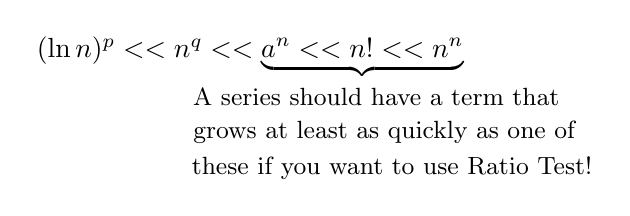
\begin{tikzpicture}
        \node at (0,0) {
          $(\ln n)^p << n^q << \underbrace{a^n << n! << n^n}$
        };
        \node at (1.6,-.5) {\small{A series should have a term that}};
         \node at (1.7,-.95) {\small{grows at least as quickly as one of}};
         \node at (1.8,-1.4) {\small{these if you want to use Ratio Test! }};
      \end{tikzpicture}
  \end{image}

\begin{question}
Without performing any calculations, determine which of the following series would the Ratio Test would be conclusive.  That is, which of the following would either converge or diverge as a consequence of the Ratio Test?
\begin{selectAll}
\choice{$\sum_{k=1}^{\infty} \frac{\sqrt{k^2+4}}{k^5+2\sqrt{k}+1}$}
\choice[correct]{$\sum_{k=1}^{\infty} \frac{\ln(k) +k^2}{k!}$}
\choice[correct]{$\sum_{k=1}^{\infty} \frac{k^{10}}{5^k}$}
\choice{$\sum_{k=1}^{\infty} \frac{(\ln k)^{80}}{k^5}$}
\choice[correct]{$\sum_{k=1}^{\infty} \frac{2^k}{k^k}$}
\end{selectAll}
\end{question}


\section{Summary}
We summarize the important results about the ratio test.  Consider a series $\sum_{k=k_0}^{\infty} a_k$.


\begin{itemize}
\item If $p(x)$ is a polynomial, $\lim_{n \to \infty} \frac{p(n+1)}{p(n)} = 1$, so the ratio test will only be conclusive if $a_k$ has a factor that grows at least exponentially (according to the growth rates results).
\item To use the test, set $L = \lim_{n \to \infty} \left| \frac{a_{n+1}}{a_n} \right|.$ 

\begin{itemize}
  \item If $0 \leq L < 1$, then the series converges.
  \item If $L>1$ or $r$ is infinite, then the series diverges.
  \item If $L = 1$, the test is inconclusive; the series could diverge or converge.
  \end{itemize}

\item In the case where a series converges, the ratio test gives no information about the value of the series.
 \end{itemize}
 
\end{document}


